\chapter{Fundamentos teóricos}
\label{cap:fundamentos}

\section{El cuerpo \texorpdfstring{$\mathbb{F}_2$}{F2}}

Todas las operaciones de un LFSR trabajan sobre el cuerpo $\mathbb{F}_2$, que es
el cuerpo de Galois con dos elementos: $\{0, 1\}$. Las operaciones son las de suma
y producto habituales pero reducidas módulo 2:

\begin{align*}
  0 + 0 = 0, \quad 0 + 1 = 1, \quad 1 + 1 = 0 \\
  0 \cdot 0 = 0, \quad 0 \cdot 1 = 0, \quad 1 \cdot 1 = 1
\end{align*}

La suma en $\mathbb{F}_2$ coincide con la operación XOR a nivel de bit, que es la operación
básica de cualquier implementación hardware o software de un LFSR.

Con este cuerpo se pueden construir también polinomios. Un polinomio sobre $\mathbb{F}_2$
es una expresión de la forma

\[
  p(x) = a_n x^n + a_{n-1} x^{n-1} + \cdots + a_1 x + a_0, \quad a_i \in \{0, 1\}
\]

y las operaciones entre polinomios se realizan igual que en los polinomios ordinarios, pero
los coeficientes se suman y multiplican en $\mathbb{F}_2$. Por ejemplo:

\[
  (x^3 + x + 1) + (x^3 + x^2) = x^2 + x + 1
\]

porque $1 + 1 = 0$ en $\mathbb{F}_2$.

La multiplicación funciona como es habitual, pero reduciendo coeficientes módulo 2:

\[
  (x^2 + x + 1)(x + 1) = x^3 + x^2 + x + x^2 + x + 1 = x^3 + 1
\]

Los términos $x^2 + x^2 = 0$ y $x + x = 0$ se cancelan por la aritmética de
$\mathbb{F}_2$. Un detalle que conviene tener presente: en $\mathbb{F}_2$ sumar y restar
es lo mismo, porque $-1 = 1$.

También se puede dividir polinomios. Dados $a(x)$ y $b(x)$ con $b(x) \neq 0$, siempre
existen un cociente $q(x)$ y un resto $r(x)$ únicos tales que

\[
  a(x) = q(x) \cdot b(x) + r(x), \quad \text{con } \deg(r) < \deg(b)
\]

\begin{ejemplo}
Dividamos $a(x) = x^4 + x^3 + 1$ entre $b(x) = x^2 + x + 1$. Haciendo la división
larga en $\mathbb{F}_2$:

\[
  x^4 + x^3 + 1 = (x^2 + 1)(x^2 + x + 1) + x
\]

Se puede comprobar multiplicando: $(x^2 + 1)(x^2 + x + 1) = x^4 + x^3 + x^2 + x^2 +
x + 1 = x^4 + x^3 + x + 1$, y sumando el resto $x$ se recupera $x^4 + x^3 + 1$.
El cociente es $q(x) = x^2 + 1$ y el resto $r(x) = x$.
\end{ejemplo}

A partir de la división se define el \textbf{máximo común divisor} de dos polinomios
mediante el algoritmo de Euclides: se va dividiendo sucesivamente hasta llegar a resto
cero, y el último resto no nulo es el MCD. Dos polinomios son coprimos si su MCD es 1.

\begin{ejemplo}
Calculemos $\gcd(x^4 + x + 1, \; x^3 + x + 1)$ en $\mathbb{F}_2[x]$.

Primera división: $x^4 + x + 1 = x \cdot (x^3 + x + 1) + (x^2 + 1)$.

Se comprueba: $x(x^3 + x + 1) = x^4 + x^2 + x$, y sumando el resto
$x^4 + x^2 + x + x^2 + 1 = x^4 + x + 1$.

Segunda división: $x^3 + x + 1 = x \cdot (x^2 + 1) + 1$.

Se comprueba: $x(x^2 + 1) = x^3 + x$, y sumando el resto $x^3 + x + 1 = x^3 + x + 1$.

Tercera división: $x^2 + 1 = (x^2 + 1) \cdot 1 + 0$.

El último resto no nulo es 1, así que $\gcd(x^4 + x + 1, \; x^3 + x + 1) = 1$:
los dos polinomios son coprimos. Esto tiene sentido porque ambos son primitivos (de
grados 4 y 3, respectivamente), y un polinomio irreducible solo puede tener como
divisores a 1 y a sí mismo.
\end{ejemplo}

La aritmética modular con polinomios funciona igual que con enteros. Trabajar módulo
un polinomio $p(x)$ de grado $n$ significa reducir siempre el resultado quedándose con
el resto de dividir por $p(x)$. Si $p(x)$ es irreducible, el conjunto de restos posibles
forma un cuerpo con $2^n$ elementos, que se denota $\mathbb{F}_{2^n}$. Y si además
$p(x)$ es primitivo, el elemento $x$ genera todo el grupo multiplicativo de ese cuerpo:
las potencias $x^0, x^1, \ldots, x^{2^n-2}$ recorren todos los elementos no nulos de
$\mathbb{F}_{2^n}$. Esta es precisamente la conexión entre los polinomios primitivos y
el periodo máximo de un LFSR.

Antes de definir los polinomios que realmente nos interesan para los LFSR, hay que
introducir el concepto de irreducibilidad. Un polinomio $p(x)$ de grado $n \geq 1$
sobre $\mathbb{F}_2$ es \textbf{irreducible} si no se puede escribir como producto de
dos polinomios de grado menor. Es básicamente la misma idea que un número primo, pero
para polinomios. Por ejemplo, $x^2 + x + 1$ es irreducible sobre $\mathbb{F}_2$:
evaluando en los dos únicos elementos del cuerpo,

\begin{align*}
  p(0) &= 0 + 0 + 1 = 1 \neq 0 \\
  p(1) &= 1 + 1 + 1 = 1 \neq 0
\end{align*}

no tiene raíces y, como es de grado 2, eso basta para concluir que es irreducible.
En cambio, $x^2 + 1$ no lo es: en $\mathbb{F}_2$ se factoriza como $(x+1)^2$,
porque $-1 = 1$ en este cuerpo.

Dentro de los irreducibles, los que nos interesan para los LFSR son los
\textbf{polinomios primitivos}. Un polinomio irreducible $p(x)$ de grado $n$ es
primitivo si el orden del elemento $x$ en el cuerpo cociente
$\mathbb{F}_2[x]/p(x)$ es exactamente $2^n - 1$, es decir, el máximo posible. En
términos prácticos: si usamos un polinomio primitivo como retroalimentación de un LFSR,
el registro va a pasar por todos los $2^n - 1$ estados no nulos antes de repetirse.

No todo polinomio irreducible es primitivo. El polinomio $x^4 + x^3 + x^2 + x + 1$
es irreducible sobre $\mathbb{F}_2$, pero el orden de $x$ en su cuerpo cociente es
solo 5, no $2^4 - 1 = 15$. Si construimos un LFSR con este polinomio, su periodo será
5 en vez de 15. En cambio, $x^4 + x + 1$ sí es primitivo y da periodo máximo.

La tabla~\ref{tab:primitivos} recoge un polinomio primitivo para cada grado de 2 a 7,
junto con el periodo que induce y el total de primitivos de ese grado. Para cada grado
hay varios en general, pero basta con conocer uno.

\begin{table}[ht]
\centering
\begin{tabular}{cccc}
\hline
\textbf{Grado} & \textbf{Polinomio primitivo} & \textbf{Periodo} & \textbf{Nº de primitivos} \\
\hline
2 & $x^2 + x + 1$           & 3    & 1 \\
3 & $x^3 + x + 1$           & 7    & 2 \\
4 & $x^4 + x + 1$           & 15   & 2 \\
5 & $x^5 + x^2 + 1$         & 31   & 6 \\
6 & $x^6 + x + 1$           & 63   & 6 \\
7 & $x^7 + x^6 + 1$         & 127  & 18 \\
\hline
\end{tabular}
\caption{Un polinomio primitivo representativo para cada grado, con el periodo que induce
y el número total de primitivos de ese grado sobre $\mathbb{F}_2$.}
\label{tab:primitivos}
\end{table}

A medida que el grado crece, el número de primitivos aumenta rápido y la proporción
respecto al total de irreducibles se mantiene razonable, así que encontrar uno no es
un problema en la práctica. Los polinomios que uso en la implementación son exactamente
los de esta tabla y algunos de grado mayor para los generadores.

\section{Registros de desplazamiento con retroalimentación lineal}

\subsection{Definición y funcionamiento}

Un LFSR de grado $n$ es un registro de $n$ celdas binarias $s_{n-1}, s_{n-2}, \ldots, s_0$
con un mecanismo de realimentación. En cada ciclo de reloj, el contenido del registro se
desplaza una posición y se calcula un nuevo bit que se introduce por un extremo:

\[
  s_{-1} = c_1 s_0 \oplus c_2 s_1 \oplus \cdots \oplus c_n s_{n-1}
\]

donde los coeficientes $c_i \in \{0, 1\}$ definen el \textbf{polinomio de retroalimentación}:

\[
  p(x) = x^n + c_1 x^{n-1} + \cdots + c_{n-1} x + c_n
\]

El bit de salida en cada ciclo es el bit que se desplaza fuera del registro, es decir,
$s_0$. La figura~\ref{fig:lfsr3} muestra la estructura de un LFSR de grado 3 con
polinomio $p(x) = x^3 + x + 1$.

\begin{figure}[ht]
\centering
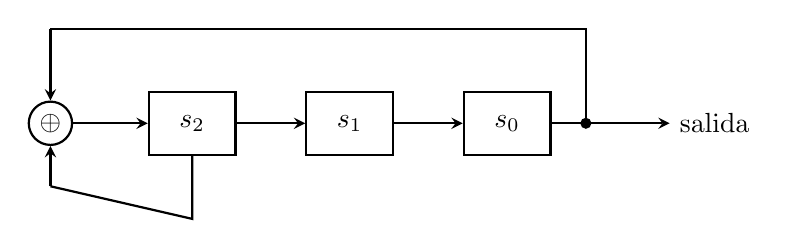
\begin{tikzpicture}[
    cell/.style={draw, minimum width=1.1cm, minimum height=0.8cm},
    xor/.style={draw, circle, minimum size=0.55cm, inner sep=0pt},
    >=stealth, thick
]
\node[cell] (s2) at (0,0) {$s_2$};
\node[cell] (s1) at (2,0) {$s_1$};
\node[cell] (s0) at (4,0) {$s_0$};

\node[xor] (xor1) at (-1.8,0) {$\oplus$};

\draw[->] (xor1) -- (s2);
\draw[->] (s2) -- (s1);
\draw[->] (s1) -- (s0);
\draw[->] (s0.east) -- ++(1.5,0) node[right] {salida};

\coordinate (split) at (5,0);
\fill (split) circle (2pt);
\draw (split) -- ++(0,1.2) -- (-1.8,1.2);
\draw[->] (-1.8,1.2) -- (xor1.north);

\draw (s2.south) -- ++(0,-0.8) -- (-1.8,-0.8);
\draw[->] (-1.8,-0.8) -- (xor1.south);
\end{tikzpicture}
\caption{LFSR de grado 3 con polinomio $p(x) = x^3 + x + 1$. Los coeficientes no nulos conectan las celdas $s_0$ y $s_2$ con la puerta XOR
de retroalimentación.}
\label{fig:lfsr3}
\end{figure}

\begin{ejemplo}
Sea un LFSR de grado 3 con polinomio de retroalimentación $p(x) = x^3 + x + 1$,
que corresponde a los coeficientes no nulos $\{3, 1\}$. Con estado inicial $(1, 0, 0)$, el bit de
retroalimentación en cada ciclo es $s_{-1} = s_0 \oplus s_2$, y el bit de salida
es el que se desplaza fuera por la derecha. La evolución completa del registro es:

\begin{center}
\begin{tabular}{cccccc}
\hline
\textbf{Ciclo} & \textbf{$s_2$} & \textbf{$s_1$} & \textbf{$s_0$} &
\textbf{Retroalimentación} & \textbf{Salida} \\
\hline
0 (inicial) & 1 & 0 & 0 & — & — \\
1 & 1 & 1 & 0 & $0 \oplus 1 = 1$ & 0 \\
2 & 1 & 1 & 1 & $0 \oplus 1 = 1$ & 0 \\
3 & 0 & 1 & 1 & $1 \oplus 1 = 0$ & 1 \\
4 & 0 & 0 & 1 & $1 \oplus 0 = 1$ & 1 \\
5 & 1 & 0 & 0 & $1 \oplus 0 = 1$ & 1 \\
6 & 0 & 1 & 0 & $0 \oplus 1 = 1$ & 0 \\
7 & 1 & 0 & 0 & $0 \oplus 0 = 0$ & 1 \\
\hline
\end{tabular}
\end{center}

En el ciclo 7 el registro vuelve al estado inicial $(1, 0, 0)$, completando el periodo.
La secuencia generada es $\{0, 0, 1, 1, 1, 0, 1\}$, de longitud $2^3 - 1 = 7$, lo
que confirma que $p(x) = x^3 + x + 1$ es primitivo sobre $\mathbb{F}_2$.
\end{ejemplo}

\subsection{Periodo y secuencias de longitud máxima}

La secuencia de salida de un LFSR es siempre periódica. El registro tiene $n$ celdas
binarias, lo que da $2^n$ estados posibles. El estado todo-ceros es un punto fijo
la retroalimentación XOR daría siempre 0, así que quedan $2^n - 1$ estados útiles.
Como el número de estados es finito, tarde o temprano el registro vuelve a un estado
que ya visitó, y a partir de ahí la secuencia se repite.

El periodo concreto depende del polinomio de retroalimentación. Si es primitivo, el
periodo es exactamente $2^n - 1$: el LFSR recorre todos los estados no nulos. Si es
irreducible pero no primitivo, el periodo divide a $2^n - 1$ pero se queda corto. Y
si el polinomio es reducible, la cosa es todavía peor.

\begin{ejemplo}
\label{ej:periodo}
Retomando el ejemplo anterior: un LFSR de grado 4 con el polinomio
$x^4 + x^3 + x^2 + x + 1$ (irreducible, no primitivo) tiene periodo 5. Con
$x^4 + x + 1$ (primitivo), el periodo sube a $2^4 - 1 = 15$, el máximo. La diferencia
viene únicamente del polinomio elegido.
\end{ejemplo}

Las secuencias que alcanzan el periodo máximo $2^n - 1$ se llaman \textbf{secuencias de
longitud máxima} o \textit{m-sequences}. Golomb~\cite{golomb1967} estableció tres
propiedades que caracterizan a estas secuencias:

\begin{enumerate}
  \item \textbf{Balance}: en cada periodo completo, el número de unos supera al de
        ceros en exactamente uno. Para grado $n$, hay $2^{n-1}$ unos y $2^{n-1} - 1$
        ceros.
  \item \textbf{Rachas}: una racha es una subsecuencia maximal de bits consecutivos
        iguales. En una m-sequence, la mitad de las rachas tienen longitud 1, un cuarto
        longitud 2, un octavo longitud 3, y así sucesivamente. Para cada longitud, hay
        tantas rachas de ceros como de unos.
  \item \textbf{Autocorrelación de dos niveles}: si desplazamos la secuencia $\tau$
        posiciones y la comparamos consigo misma, la coincidencia es máxima cuando
        $\tau = 0$ y vale $-1/(2^n - 1)$ para cualquier otro desplazamiento. Esto es
        exactamente lo que esperaríamos de una secuencia verdaderamente aleatoria.
\end{enumerate}

\begin{ejemplo}
Para el LFSR de grado 5 con $p(x) = x^5 + x^2 + 1$, la m-sequence tiene periodo 31.
Contiene 16 unos y 15 ceros (balance). Las rachas se distribuyen así: 8 de longitud 1,
4 de longitud 2, 2 de longitud 3, 1 de longitud 4 y 1 de longitud 5. La autocorrelación
fuera del desplazamiento cero es $-1/31 \approx -0{,}032$, prácticamente nula.
\end{ejemplo}

Además de estos tres postulados, las m-sequences tienen otra propiedad
fundamental: la propiedad \textbf{shift-and-add}. Si sumamos (XOR) una m-sequence
consigo misma desplazada cualquier número de posiciones $\tau \neq 0$, el resultado
es la misma m-sequence pero con otro desplazamiento. Es decir, el conjunto de todas
las versiones desplazadas de una m-sequence es cerrado bajo la suma en $\mathbb{F}_2$.

Formalmente, si $\mathbf{s} = \{s_i\}$ es una m-sequence de periodo $T = 2^n - 1$ y
$\mathbf{s}^{(\tau)}$ denota la secuencia desplazada $\tau$ posiciones, entonces para
cada $\tau$ con $1 \leq \tau \leq T - 1$ existe un $\sigma$ tal que

\[
  s_i \oplus s_{i+\tau} = s_{i+\sigma} \quad \text{para todo } i
\]

\begin{ejemplo}
La m-sequence de grado 3 con $p(x) = x^3 + x + 1$ tiene periodo 7. Tomando la
secuencia $\{0, 0, 1, 1, 1, 0, 1, \ldots\}$ y desplazándola 2 posiciones se obtiene
$\{1, 1, 1, 0, 1, 0, 0, \ldots\}$. Si las sumamos bit a bit:
\[
  \{0, 0, 1, 1, 1, 0, 1\} \oplus \{1, 1, 1, 0, 1, 0, 0\} = \{1, 1, 0, 1, 0, 0, 1\}
\]
que es la misma m-sequence desplazada 5 posiciones. Cualquier otra combinación de
desplazamientos produce otro desplazamiento de la misma secuencia.
\end{ejemplo}

Esta propiedad tiene una consecuencia negativa para la seguridad: significa que
combinaciones lineales de versiones desplazadas de una m-sequence no introducen ninguna
complejidad nueva, porque el resultado sigue siendo la misma secuencia. Esto refuerza
la necesidad de usar combinaciones no lineales para construir generadores resistentes.

Otra forma de entender las m-sequences es a través de \textbf{series formales de
potencias}. La secuencia de salida $s_0, s_1, s_2, \ldots$ de un LFSR con polinomio
de retroalimentación $p(x)$ de grado $n$ se puede escribir como la serie formal

\[
  S(x) = \sum_{i=0}^{\infty} s_i x^i = \frac{g(x)}{p^*(x)}
\]

donde $p^*(x) = x^n p(x^{-1})$ es el polinomio recíproco de $p(x)$ y $g(x)$ es un
polinomio de grado menor que $n$ que depende del estado inicial. Es decir, la secuencia
infinita queda completamente descrita por una fracción racional de polinomios sobre
$\mathbb{F}_2$.

\begin{ejemplo}
Para el LFSR de grado 3 con $p(x) = x^3 + x + 1$ y estado inicial $(1, 0, 0)$:
el polinomio recíproco es $p^*(x) = x^3 \cdot p(1/x) = 1 + x^2 + x^3$.

La secuencia de salida $\{0, 0, 1, 1, 1, 0, 1, 0, 0, 1, \ldots\}$ corresponde a
la serie $S(x) = x^2 + x^3 + x^4 + x^6 + \cdots$, que se puede escribir como
\[
  S(x) = \frac{x^2}{1 + x^2 + x^3}
\]
donde $g(x) = x^2$ es el polinomio del numerador determinado por el estado inicial.
Esto captura toda la información del generador en una expresión compacta. El
denominador es el recíproco del polinomio de retroalimentación, y determina la
estructura periódica de la secuencia; el numerador solo fija la fase.
\end{ejemplo}

Esta representación como función racional es otra forma de ver por qué la secuencia
es predecible: una fracción de polinomios de grado $n$ queda determinada por $2n$
coeficientes. Berlekamp-Massey, en esencia, reconstruye esta fracción a partir de los
primeros términos de la serie.

Las tres propiedades de Golomb, la propiedad shift-and-add y la representación racional
hacen que las m-sequences estén muy bien entendidas matemáticamente. Pasan tests
estadísticos básicos, la distribución parece equilibrada, no hay patrones sospechosos en
las rachas y la autocorrelación se comporta como la de un ruido. A primera vista, la
secuencia tiene pinta de ser aleatoria.

Pero es una impresión engañosa. La complejidad lineal de una m-sequence es exactamente
$n$, el grado del LFSR, por muy largo que sea el periodo. Como veremos a continuación,
esto las hace completamente vulnerables frente a Berlekamp-Massey.

\subsection{Vulnerabilidad frente al algoritmo de Berlekamp-Massey}

A pesar de estas buenas propiedades, un LFSR solo no sirve para criptografía. El
motivo es que su complejidad lineal, como veremos en la siguiente sección, es igual a
su grado $n$. Con $2n$ bits observados de la secuencia, Berlekamp-Massey reconstruye
el polinomio de retroalimentación y el estado inicial completo.

Para hacerse una idea: un LFSR de grado 19 genera secuencias de más de medio millón
de bits, pero bastan 38 bits observados para romperlo. De ahí viene la necesidad de
usar construcciones más complejas.

\section{Complejidad lineal}

\subsection{Definición}

La \textbf{complejidad lineal} de una secuencia binaria $s = s_0, s_1, s_2, \ldots$ es la
longitud $L$ del LFSR más corto capaz de generar dicha secuencia. Se denota $\Lambda(s)$.

Formalmente, $\Lambda(s) = L$ si existe un LFSR de grado $L$ con un estado inicial
adecuado que produce la secuencia $s$, y no existe ningún LFSR de grado menor que lo
consiga.

Para una secuencia finita de longitud $N$, la complejidad lineal es siempre menor o igual
a $\lfloor N/2 \rfloor$.

Algunos casos sencillos ayudan a fijar la idea:

\begin{itemize}
  \item La secuencia todo-ceros $\{0, 0, 0, \ldots\}$ tiene $\Lambda = 0$: no hace falta
        ningún LFSR porque la secuencia es trivial.
  \item La secuencia constante $\{1, 1, 1, \ldots\}$ tiene $\Lambda = 1$: basta un LFSR
        de grado 1 con polinomio $x + 1$.
  \item La secuencia alternante $\{0, 1, 0, 1, \ldots\}$ tiene $\Lambda = 2$.
  \item Una m-sequence generada por un LFSR de grado $n$ tiene $\Lambda = n$: no se
        puede comprimir en un LFSR más corto, pero tampoco necesita uno más largo.
\end{itemize}

El caso interesante es el de una secuencia verdaderamente aleatoria. Si tomamos una
secuencia de $N$ bits generada de forma aleatoria uniforme, su complejidad lineal esperada
es aproximadamente $N/2$. Esto establece una referencia natural: para que un generador
sea criptográficamente aceptable, su complejidad lineal debería estar en ese entorno.
Si está muy por debajo de $N/2$, la secuencia tiene más estructura lineal de la que
debería y es potencialmente vulnerable.

\subsection{Importancia criptográfica}

La complejidad lineal es la medida más directa de lo resistente que es una secuencia
frente a Berlekamp-Massey. Si una secuencia tiene complejidad lineal $L$, se puede
reconstruir a partir de $2L$ bits, así que cuanto mayor sea $L$, más bits necesita
observar un atacante.

Para que una secuencia sea aceptable criptográficamente, su complejidad lineal tiene
que ser grande (idealmente del orden de la mitad de la longitud del periodo) y además
tiene que ser estable: que añadir unos pocos bits no reduzca drásticamente la
complejidad.

Esta segunda condición se formaliza con el \textbf{perfil de complejidad lineal},
$\Lambda_0, \Lambda_1, \Lambda_2, \ldots$, donde $\Lambda_i$ es la complejidad lineal del
prefijo $s_0, s_1, \ldots, s_{i-1}$. Si el generador es bueno, el perfil crece de forma
más o menos regular, manteniéndose cerca de la recta $N/2$. Si tiene saltos bruscos o se
estanca en valores bajos durante muchos bits, es señal de que la secuencia tiene una
estructura explotable.

Para una m-sequence el perfil es revelador: se estabiliza en $\Lambda = n$ tras procesar
apenas $2n$ bits y después no vuelve a cambiar. El LFSR queda completamente determinado
muy pronto. En una secuencia aleatoria ideal, por el contrario, el perfil iría subiendo
gradualmente hasta $N/2$, sin estancarse.

\begin{ejemplo}
Veamos los perfiles de complejidad lineal para dos secuencias distintas de 14 bits. La
primera es la salida de un LFSR de grado 3, la segunda es una secuencia elegida para
tener complejidad alta.

\medskip

Secuencia~A (m-sequence, grado 3): $\{0, 0, 1, 1, 1, 0, 1, 0, 0, 1, 1, 1, 0, 1\}$

\begin{center}
\begin{tabular}{c|cccccccccccccc}
$N$ & 1 & 2 & 3 & 4 & 5 & 6 & 7 & 8 & 9 & 10 & 11 & 12 & 13 & 14 \\
\hline
$\Lambda_N$ & 0 & 0 & 2 & 3 & 3 & 3 & 3 & 3 & 3 & 3 & 3 & 3 & 3 & 3 \\
\end{tabular}
\end{center}

La complejidad sube a 3 con el cuarto bit y no vuelve a moverse. A partir de ese
momento, Berlekamp-Massey ya ha identificado el LFSR: todos los bits restantes son
predecibles.

\medskip

Secuencia~B (secuencia con más estructura): $\{1, 0, 1, 1, 0, 0, 1, 0, 1, 1, 1, 0, 0, 1\}$

\begin{center}
\begin{tabular}{c|cccccccccccccc}
$N$ & 1 & 2 & 3 & 4 & 5 & 6 & 7 & 8 & 9 & 10 & 11 & 12 & 13 & 14 \\
\hline
$\Lambda_N$ & 1 & 1 & 2 & 2 & 3 & 3 & 4 & 4 & 5 & 5 & 6 & 6 & 7 & 7 \\
\end{tabular}
\end{center}

Aquí el perfil crece de forma regular, manteniéndose siempre cerca de $N/2$. Cada dos
bits, la complejidad sube en uno: exactamente lo que esperaríamos de una secuencia sin
estructura lineal explotable.

\medskip

La diferencia entre ambos perfiles ilustra lo que buscamos en un buen generador: un
perfil que crezca de forma sostenida, sin estancarse en valores bajos. Cuando en el
capítulo~\ref{cap:analisis} analicemos los generadores, los perfiles de complejidad
lineal serán una de las herramientas principales para compararlos.
\end{ejemplo}

\subsection{El algoritmo de Berlekamp-Massey}
\label{sec:berlekamp-massey}

El algoritmo de Berlekamp-Massey \cite{massey1969} resuelve el problema de encontrar el
LFSR más corto para una secuencia dada. Fue propuesto originalmente por Berlekamp en el
contexto de la decodificación de códigos BCH, y adaptado por Massey para el análisis de
secuencias en 1969.

El algoritmo funciona de forma iterativa. Mantiene un polinomio de conexión candidato
$C(x)$ y lo va actualizando cada vez que encuentra una discrepancia entre lo que
predice el LFSR actual y lo que realmente se observa en la secuencia. La condición
de actualización es:

\[
  d_i = s_i \oplus \sum_{j=1}^{L} c_j \cdot s_{i-j} \neq 0
\]

Si hay discrepancia y $2L \leq i$, es necesario aumentar la longitud del LFSR.

El procedimiento completo es el siguiente:

\begin{enumerate}
  \item Inicializar el polinomio de conexión $C(x) = 1$, un polinomio auxiliar
        $B(x) = 1$, la longitud $L = 0$ y un contador de desplazamiento $m = 1$.
  \item Para cada bit $s_i$ de la secuencia (con $i = 0, 1, \ldots, N-1$):
        \begin{enumerate}
          \item Calcular la discrepancia
                $d_i = s_i \oplus \sum_{j=1}^{L} c_j \cdot s_{i-j}$.
          \item Si $d_i = 0$: el LFSR actual predice correctamente $s_i$.
                Incrementar $m$.
          \item Si $d_i = 1$ y $2L \leq i$: el LFSR es demasiado corto. Guardar
                $T(x) = C(x)$, actualizar $C(x) \leftarrow C(x) \oplus x^m B(x)$,
                hacer $L \leftarrow i + 1 - L$, $B(x) \leftarrow T(x)$ y $m \leftarrow 1$.
          \item Si $d_i = 1$ y $2L > i$: hay discrepancia pero el LFSR ya es lo
                bastante largo. Actualizar solo
                $C(x) \leftarrow C(x) \oplus x^m B(x)$ e incrementar $m$.
        \end{enumerate}
  \item Al terminar, $L = \Lambda(s)$ y $C(x)$ es el polinomio de conexión del LFSR
        mínimo.
\end{enumerate}

El paso clave es el 2(c): cuando hay discrepancia y el LFSR actual no es lo bastante
largo, se aumenta $L$ y se guarda el polinomio anterior en $B(x)$ para futuras
correcciones. El polinomio $B(x)$ actúa como memoria de la última corrección que
cambió la longitud, y el desplazamiento $m$ controla dónde se aplica. Todo el proceso
termina en tiempo $O(N^2)$ y la longitud final es exactamente $\Lambda(s)$.

\begin{ejemplo}
Apliquemos el algoritmo a la secuencia $\{0, 0, 1, 1, 1, 0, 1\}$ generada por el LFSR
de grado 3 con $p(x) = x^3 + x + 1$. El algoritmo parte con $C(x) = 1$ y $L = 0$:

\begin{center}
\begin{tabular}{ccccl}
\hline
$i$ & $s_i$ & $d_i$ & $L$ & $C(x)$ \\
\hline
0 & 0 & 0 & 0 & $1$ \\
1 & 0 & 0 & 0 & $1$ \\
2 & 1 & 1 & 3 & $1 + x^3$ \\
3 & 1 & 1 & 3 & $1 + x + x^3$ \\
4 & 1 & 0 & 3 & $1 + x + x^3$ \\
5 & 0 & 0 & 3 & $1 + x + x^3$ \\
6 & 1 & 0 & 3 & $1 + x + x^3$ \\
\hline
\end{tabular}
\end{center}

En $i = 2$ aparece la primera discrepancia ($d_2 = 1$) y como $2L = 0 \leq 2$, el
algoritmo aumenta la longitud a $L = 3$. En $i = 3$ hay otra discrepancia, pero ahora
$2L = 6 > 3$, así que solo ajusta el polinomio sin cambiar $L$. A partir de $i = 4$ ya
no hay más discrepancias: el polinomio $C(x) = 1 + x + x^3$ reproduce correctamente
la secuencia.

El resultado es $\Lambda = 3$ con polinomio de conexión $C(x) = 1 + x + x^3$, que
coincide con el polinomio de retroalimentación $x^3 + x + 1$ del LFSR original. Con solo
4 bits procesados (hasta $i = 3$) el algoritmo ya ha convergido, y los 3 bits restantes
no hacen más que confirmar el resultado. Esto muestra por qué un LFSR solo es inseguro:
el coste de romperlo es proporcional a su grado, no a la longitud de la secuencia que
genera.
\end{ejemplo}

\section{Seguridad de secuencias cifrantes}

\subsection{Criterios de una buena secuencia}

Para que una secuencia de bits sea útil como \textit{keystream} en un cifrado de flujo
no basta con que tenga buenas propiedades estadísticas. Las condiciones que debe cumplir
son varias, y conviene tenerlas claras antes de evaluar los generadores del
capítulo~\ref{cap:generadores}:

\begin{enumerate}
  \item \textbf{Complejidad lineal alta}: la complejidad lineal determina cuántos bits
        necesita un atacante para reconstruir la secuencia con Berlekamp-Massey. Si la
        secuencia tiene longitud $N$, su complejidad lineal debería estar cerca de $N/2$,
        que es lo que esperaríamos de una secuencia verdaderamente aleatoria.
  \item \textbf{Perfil de complejidad lineal estable}: no basta con que la complejidad
        lineal final sea alta. El perfil tiene que crecer de forma sostenida conforme
        se observan más bits. Si en algún punto se estanca o cae bruscamente, un atacante
        que observe la secuencia hasta ese punto podría aprovecharlo.
  \item \textbf{Periodo largo}: el periodo tiene que ser lo bastante largo para que
        la secuencia no se repita durante el uso del cifrado. Si el periodo es corto, un
        atacante puede observar un ciclo completo y predecir todo lo que viene después.
  \item \textbf{Buenas propiedades estadísticas}: la secuencia debe parecer aleatoria
        frente a tests estadísticos. Esto incluye balance entre ceros y unos, distribución
        uniforme de bloques y ausencia de patrones detectables. Los tests NIST SP 800-22
        que usamos en el capítulo~\ref{cap:analisis} evalúan precisamente esto.
  \item \textbf{Resistencia a ataques de correlación}: si el generador combina varios
        LFSR, la salida no debe tener dependencia estadística significativa con ninguno
        de los LFSR individuales.
\end{enumerate}

Las m-sequences cumplen los puntos 3 y 4 (periodo máximo y buena estadística) pero
fallan completamente en el 1: su complejidad lineal es $n$, no $N/2$. Los generadores
que estudiaremos intentan cumplir todos estos criterios combinando LFSR de distintas
formas, cada uno con su estrategia particular.

\subsection{Funciones combinadoras}

Los generadores del capítulo~\ref{cap:generadores} combinan las salidas de varios
LFSR mediante una \textbf{función booleana} $f : \mathbb{F}_2^k \to \mathbb{F}_2$
que toma los bits de salida de $k$ registros y produce un único bit de keystream.
Las propiedades de esta función determinan en gran medida la seguridad del generador
resultante.

Toda función booleana se puede escribir de forma única como un polinomio en
$\mathbb{F}_2[x_1, \ldots, x_k]$ donde cada variable aparece con exponente 0 o 1.
Esta representación se llama \textbf{forma normal algebraica} (ANF, del inglés
\textit{Algebraic Normal Form}):

\[
  f(x_1, \ldots, x_k) = a_0 \oplus \bigoplus_{i} a_i x_i \oplus
  \bigoplus_{i < j} a_{ij} x_i x_j \oplus \cdots \oplus
  a_{12\ldots k} x_1 x_2 \cdots x_k
\]

con $a_0, a_i, a_{ij}, \ldots \in \{0, 1\}$. El \textbf{grado algebraico} de $f$ es
el grado del monomio de mayor grado con coeficiente no nulo. Las funciones de grado 1
son lineales (o afines si tienen término independiente), y como hemos visto, la
linealidad es precisamente lo que hace vulnerable a un LFSR. Una función combinadora
necesita tener un grado algebraico alto para ofrecer seguridad.

\begin{ejemplo}
El generador de Geffe~\cite{geffe1973} combina tres LFSR con la función
$f(x_1, x_2, x_3) = x_1 x_2 \oplus x_2 x_3 \oplus x_3$. Su forma normal algebraica
tiene grado 2 (el monomio de mayor grado es $x_1 x_2$). Es no lineal, pero como
veremos su grado no es lo bastante alto para resistir ataques de correlación.
\end{ejemplo}

Una propiedad básica que debe tener la función es el \textbf{balance}: una función
booleana está balanceada si produce la misma cantidad de ceros que de unos cuando se
evalúa sobre todas las $2^k$ entradas posibles. Si no está balanceada, la salida del
generador tendrá un sesgo estadístico detectable.

La propiedad más relevante para la seguridad frente a ataques de correlación es la
\textbf{inmunidad a la correlación}. Una función $f$ tiene inmunidad a la correlación
de orden $m$ si su salida es estadísticamente independiente de cualquier combinación
lineal de $m$ o menos de sus entradas. Formalmente, $f$ tiene inmunidad de orden $m$
si para todo subconjunto $S \subseteq \{1, \ldots, k\}$ con $|S| \leq m$:

\[
  \Pr\left[f(x_1, \ldots, x_k) = \bigoplus_{i \in S} x_i\right] = \frac{1}{2}
\]

donde la probabilidad se toma sobre todas las entradas uniformemente distribuidas.
Si la inmunidad es 0, existe al menos una entrada individual con la que la salida
tiene correlación distinta de cero, y un atacante puede aprovecharla para aislar
ese LFSR y atacarlo por separado.

Siegenthaler~\cite{siegenthaler1985} demostró una cota que limita las propiedades
que una función combinadora puede tener a la vez. Si $f$ es una función booleana
balanceada de $k$ variables con inmunidad a la correlación de orden $m$ y grado
algebraico $d$, entonces:

\[
  m + d \leq k
\]

Esto establece un compromiso inevitable: si la función tiene inmunidad alta (resiste
ataques de correlación), su grado algebraico tiene que ser bajo, lo que la expone a
ataques algebraicos. Y al revés: un grado algebraico alto obliga a una inmunidad a la
correlación baja. Diseñar un buen generador requiere encontrar un equilibrio entre
ambas propiedades.

\begin{ejemplo}
La función de Geffe $f(x_1, x_2, x_3) = x_1 x_2 \oplus x_2 x_3 \oplus x_3$ tiene
$k = 3$ variables y grado algebraico $d = 2$. Según la cota de Siegenthaler, podría
tener hasta inmunidad $m = 1$ (ya que $1 + 2 = 3 = k$). Sin embargo, en la práctica
su inmunidad es $m = 0$: la salida coincide con $x_1$ el 75\% de las veces y con
$x_3$ también el 75\%. El diseño de Geffe ni siquiera alcanza el límite teórico que
permite la cota.
\end{ejemplo}

Esta cota ayuda a entender por qué diseñar generadores basados en LFSR es complicado:
no se pueden maximizar todas las propiedades de seguridad a la vez, y cada construcción
tiene que elegir dónde hacer las concesiones. Los generadores del
capítulo~\ref{cap:generadores} ilustran distintas formas de abordar ese compromiso.

\subsection{Ataques a generadores basados en LFSR}

Un atacante que observa parte de la secuencia de salida tiene varias estrategias para
intentar recuperar el estado interno o predecir los bits siguientes. Las principales
son:

\textbf{Ataque directo con Berlekamp-Massey.} Es el más inmediato: aplicar el
algoritmo directamente a la secuencia observada. Si la complejidad lineal del generador
es $L$, bastan $2L$ bits para recuperar el polinomio de conexión equivalente. Funciona
contra cualquier generador cuya complejidad lineal sea baja en proporción a la longitud
de la secuencia. Por eso medir la complejidad lineal es lo primero que hacemos al
analizar cada generador.

\textbf{Ataques de correlación.} Propuestos por Siegenthaler~\cite{siegenthaler1985},
explotan la dependencia estadística entre la salida del generador y la salida de alguno
de los LFSR internos. Si la función de combinación tiene un sesgo (por ejemplo, si
la salida coincide con uno de los LFSR el 75\% de las veces en lugar del 50\%
esperado), un atacante puede aislar ese LFSR y atacarlo por separado con un esfuerzo
mucho menor que la fuerza bruta sobre todo el estado. El generador de Geffe es el caso
clásico: su función de combinación tiene correlación $0{,}75$ con dos de los tres LFSR,
lo que lo hace vulnerable a este tipo de ataque.

\textbf{Ataques algebraicos.} En vez de buscar correlaciones estadísticas, plantean un
sistema de ecuaciones sobre $\mathbb{F}_2$ que relaciona los bits de salida con los bits
del estado interno. Courtois y Meier~\cite{courtois2003} mostraron que muchos generadores
basados en LFSR son vulnerables si la función de combinación tiene grado algebraico bajo,
porque el sistema resultante se puede resolver eficientemente. Estos ataques son más
recientes y más generales que los de correlación, pero también más complejos de
implementar.

\textbf{Fuerza bruta sobre el estado.} El ataque más simple: probar todos los posibles
estados iniciales hasta encontrar uno que reproduzca la secuencia observada. Si el
generador usa LFSR con grados $n_1, n_2, \ldots, n_k$, el espacio de búsqueda tiene
tamaño $2^{n_1 + n_2 + \cdots + n_k}$, que para tamaños razonables es inabordable.
Este ataque sirve como referencia: si alguno de los otros reduce el esfuerzo por debajo
de la fuerza bruta, el generador tiene una debilidad real.

En este trabajo nos centramos en el análisis de la complejidad lineal con
Berlekamp-Massey y en la evaluación estadística con los tests NIST. Los ataques de
correlación y algebraicos se mencionan donde son relevantes (especialmente al hablar
del generador de Geffe) pero no los implementamos.

\subsection{Tests estadísticos}

Los criterios de seguridad de la sección anterior son propiedades teóricas, pero en la
práctica hace falta una forma concreta de comprobar si una secuencia se comporta como
aleatoria. Para eso existen las baterías de tests estadísticos, siendo la más
utilizada la del estándar NIST SP 800-22~\cite{nist2010}.

La idea detrás de cada test es un contraste de hipótesis. La hipótesis nula $H_0$ es
que la secuencia ha sido generada por un proceso verdaderamente aleatorio. El test
analiza alguna propiedad concreta de la secuencia (balance de bits, longitud de las
rachas, rango de submatrices, componentes frecuenciales, etc.) y calcula un
\textbf{p-valor} que mide cuánto se desvía el valor observado de lo que se esperaría
bajo $H_0$.

Si el p-valor es mayor que el nivel de significación $\alpha$ (en este trabajo se usa
$\alpha = 0{,}01$), no hay evidencia suficiente para rechazar la aleatoriedad: la
secuencia supera el test. Si es menor, la secuencia muestra un comportamiento que
sería muy improbable en una secuencia aleatoria real, y el test la marca como
sospechosa para esa propiedad concreta.

Hay que tener en cuenta que superar un test no demuestra que la secuencia sea
aleatoria. Simplemente significa que no se ha detectado una desviación en la propiedad
que ese test evalúa. Cuantos más tests pase una secuencia, mayor confianza se tiene en
que no presenta debilidades estadísticas evidentes, pero la ausencia de detección no es
una garantía de seguridad. Un generador podría pasar todos los tests estadísticos y
seguir siendo vulnerable a un ataque de correlación o algebraico, que explota la
estructura interna del generador y no solo las propiedades estadísticas de la salida.

El estándar NIST SP 800-22 define quince tests, cada uno orientado a detectar un tipo
de desviación distinto. Algunos son relativamente sencillos, como el test de frecuencia,
que comprueba si la proporción de ceros y unos se acerca al 50\%. Otros son más
específicos: el test espectral aplica la transformada discreta de Fourier para buscar
periodicidades ocultas, y el test de complejidad lineal mide directamente si la
secuencia se puede comprimir en un LFSR más corto de lo esperado. Cada test captura
un aspecto diferente de la aleatoriedad, y ninguno por sí solo es suficiente.

En el capítulo~\ref{cap:analisis} se detallan los ocho tests seleccionados para este
trabajo, se presentan los p-valores obtenidos por cada generador y se comparan los
resultados para determinar cuáles superan la batería completa y cuáles muestran
debilidades detectables.
